\documentclass[11pt]{article}

% ====================================================
% PACKAGES
% ====================================================
\usepackage[margin=1in, headheight=13.6pt]{geometry}
\usepackage[T1]{fontenc}
\usepackage{lmodern}
\usepackage{microtype}
\usepackage{setspace}
\usepackage{amsmath, amssymb, mathtools}
\usepackage{siunitx}

\usepackage{graphicx}
\usepackage{float}
\usepackage{subcaption}

\usepackage{enumitem}
\usepackage{booktabs}
\usepackage{longtable}
\usepackage{array}

\usepackage{xcolor}
\usepackage{hyperref}

\usepackage{fancyhdr}
\usepackage{lastpage}

\usepackage{indentfirst}
\usepackage[justification=centering]{caption}

\pagestyle{fancy}
\fancyhf{}
\lhead{\Assignment\ |\ \course}
\rhead{\Name\ |\ \today}
\cfoot{Page \thepage\ of~\pageref{LastPage}}

\hypersetup{
    colorlinks,
    linkcolor={red!50!black},
    citecolor={blue!50!black},
    urlcolor={blue!80!black}
}

\newcommand{\Name}{Arael Anaya}
\newcommand{\Assignment}{3.6 Mobility Solution}
\newcommand{\course}{Space Robotics}

\begin{document}

\noindent\textbf{\large Mobility Solution: Four-Wheel Differential Drive on a Single-Pivot Rocker}

\bigskip

% ====================================================
\section*{I. Why Wheels}

Europa's surface is fractured, chaotic terrain, sitting at \SI{90}{K} under \SI{1.314}{m/s^2} of gravity. The
mission needs the rover to build a spatially continuous subsurface profile along a track. REQ.03.01 calls for a
radar trace every \SI{100}{m} or better along a single transect, and REQ.06.01 requires a sounding stop at each
of those intervals. A hopper or a legged walker produces discrete samples, and every landing creates a gap where
the localization solution has to start over. Wheels produce a continuous odometry signal, and that continuity is
what the whole \SI{\pm 0.5}{m} localization budget in REQ.02.01 depends on.

Low gravity favors hopping and legged locomotion on paper. A hop costs little energy at \SI{1.3}{m/s^2}, and legs
manage fractured blocks more gracefully than a rigid wheel does. Both mechanisms hinge on a single impact landing
correctly, every time. A hop that lands wrong on a \SI{90}{K} ice block can end the mission on the spot, and the
\SI{44}{min} one-way delay leaves no window for Earth to step in before the damage is done. A wheeled rocker
degrades slowly, bearing by bearing, over many sols. When the recovery loop runs that long, that slow failure
mode is worth more than the energy a hop would save.

\bigskip

% ====================================================
\section*{II. Configuration}

Four independently driven wheels ride on a single-pivot rocker, with no steering actuators. The chassis is the
\SI{0.90}{m} $\times$ \SI{0.60}{m} equipment deck already carried in the mass budget, held \SI{0.35}{m} above
the surface so the belly-mounted sounder keeps its standoff. The wheelbase measures \SI{0.70}{m} and the track
\SI{0.80}{m}. Four tapered landing struts get jettisoned after checkout, leaving only the wheels in contact with
the ice during the survey.

\begin{enumerate}[label=\alph*., leftmargin=*]
    \item \textbf{Wheels.} \SI{0.32}{m} in diameter, \SI{0.20}{m} wide, a rigid aluminum rim carrying 24
    hardened cleats. The contact path stays bare metal, since anything compliant would degrade fast under a
    \SI{90}{K} soak and the thermal cycling that follows.

    \item \textbf{Suspension.} One rocker pivot sits on the chassis belly centerline, with bent arms and elbow
    joints running out to each hub. A rocker-bogie layout, six wheels split across two bogies, would climb
    better. It also adds two actuators and two thermal isolation paths, on top of a mass budget already sitting
    at \SI{136.9}{kg} against a \SI{147.25}{kg} cap.

    \item \textbf{Steering.} Differential drive handles it. Opposing wheel rates rotate the chassis about the
    rocker pivot, so every heading change is a deliberate skid across the ice.

    \item \textbf{Speed.} Commanded speed is \SI{2}{cm/s}, driven in arcs no longer than \SI{5}{m}.
\end{enumerate}

\begin{figure}[H]
    \centering
    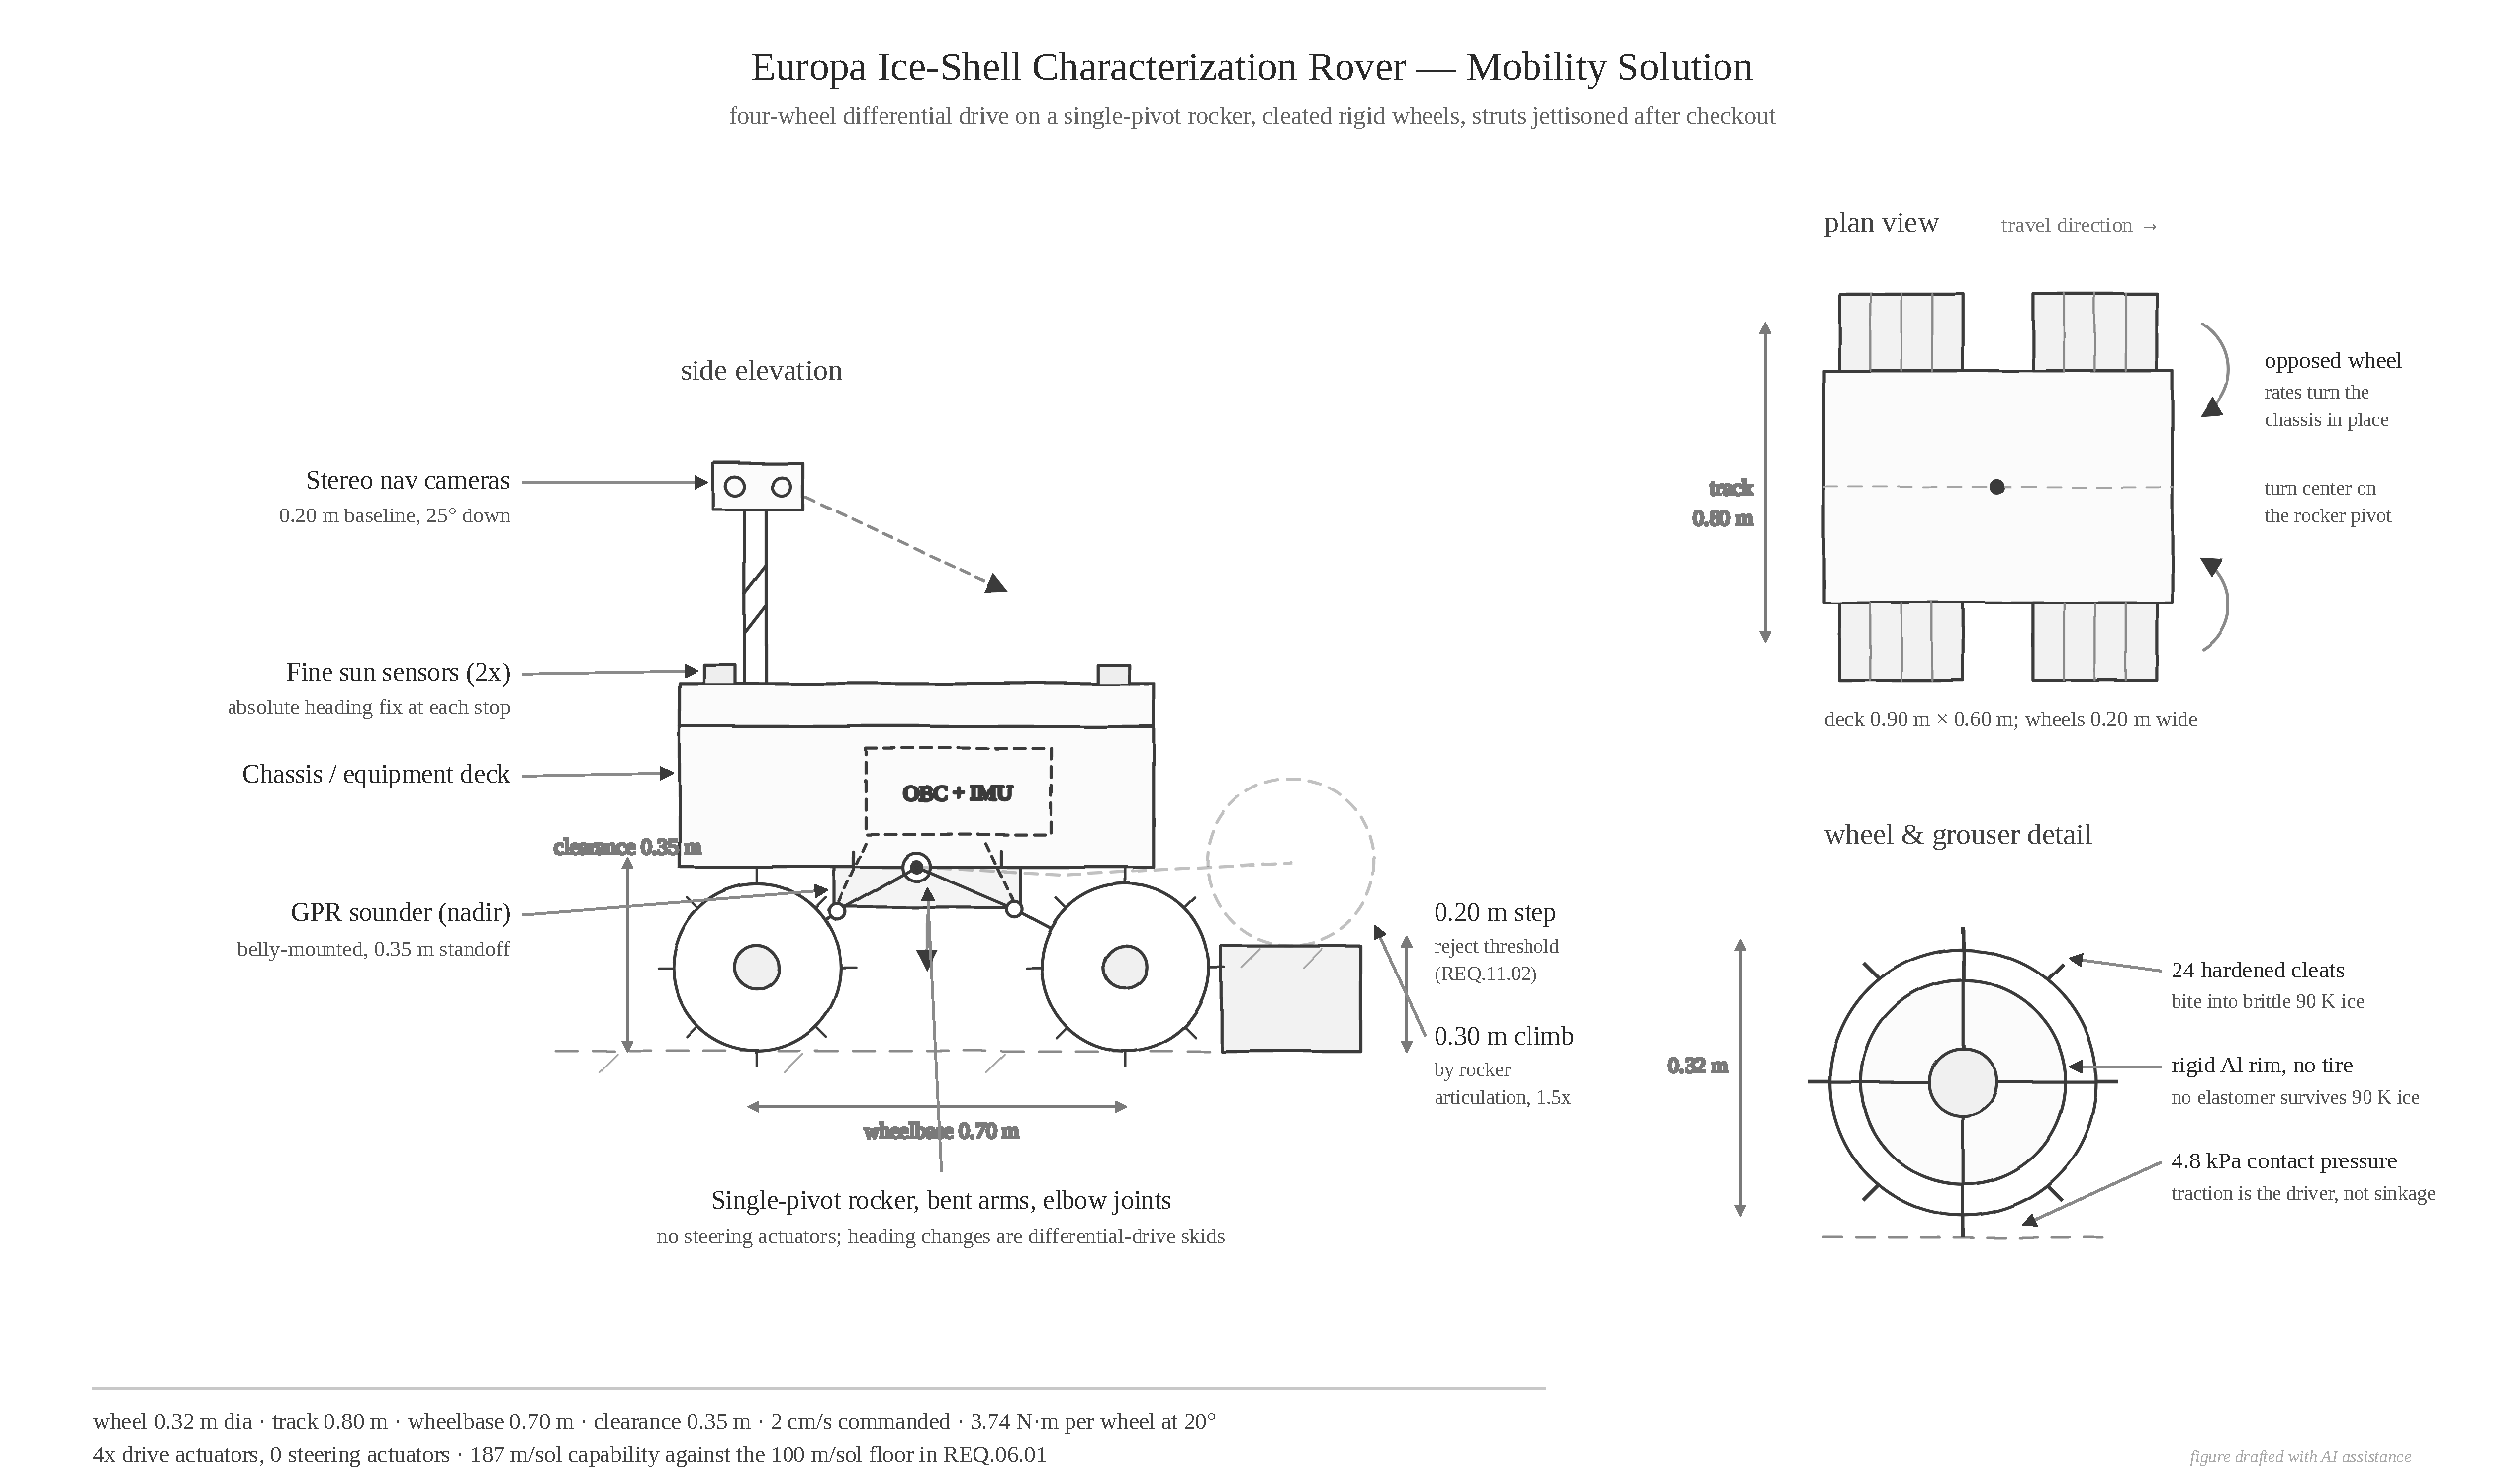
\includegraphics[width=\textwidth]{3_6_mobilitySketch_araelAnaya.pdf}
    \caption{Mobility solution: side elevation, plan view, and wheel detail.}
\end{figure}

\bigskip

% ====================================================
\section*{III. Traction and Load}

Take the mass budget at its contingency cap, \SI{147.25}{kg}. On Europa that weighs
$147.25 \times 1.314 = \SI{193.5}{N}$, \SI{48.4}{N} per wheel. Spread across a contact patch of about
\SI{0.20}{m} $\times$ \SI{0.05}{m}, that comes to \SI{4.8}{kPa}. Water ice has a compressive strength in the
megapascals, well above that number, so the wheels don't need Mars-style flotation sizing to avoid sinking in.
Their job is generating shear.

Tractive force needed to hold the \SI{20}{\degree} slope limit that REQ.03.02 already imposes, with a rolling
resistance coefficient of \num{0.15}:
\[
F = W\left(\sin\SI{20}{\degree} + 0.15\cos\SI{20}{\degree}\right)
  = 193.5 \times (0.342 + 0.141) = \SI{93.4}{N}.
\]
That force works out to \SI{23.4}{N} per wheel, \SI{3.74}{N.m} at a \SI{0.16}{m} radius. At \SI{2}{cm/s} the
useful mechanical power comes to just \SI{1.87}{W}. Nearly all of the \SI{84}{W} peak already budgeted for the
four drive motors covers breakout torque and gearbox drag at \SI{90}{K}, where stiff lubricant dominates the
load; moving the rover itself barely registers against that number. REQ.09.02 preheats the actuators above
\SI{-40}{\degreeCelsius} before any commanded motion for the same reason.

The available shear favors this design, for a reason specific to Europa. Ice turns slippery near its melting
point because contact pressure forms a thin meltwater film. At \SI{90}{K} that film doesn't form, and the
friction coefficient for a hard slider on ice climbs toward \numrange{0.5}{0.7}, far above the \num{0.05} you'd
measure on a temperate glacier~\cite{kietzig}. Using \num{0.5}, the limiting slope comes to \SI{26.6}{\degree}
against the required \SI{20}{\degree}, so the cleats carry margin without needing an aggressive grouser height.
Europa's ice behaves like brittle rock at this temperature, which helps traction and wears at the cleats, so the
cleats are separate hardened inserts bolted onto the rim.

Per-sol distance comes in well above the requirement. Four hours of drive time at \SI{2}{cm/s}, with a 65\,\%\
duty cycle after subtracting stops for imaging and hazard assessment, works out to \SI{187}{m} against the
\SI{100}{m} floor in REQ.06.01. REQ.06.01 only demands an average rate of \SI{6.9}{mm/s}, so hazard rejection
and the sounding cadence set the pace of the traverse, well before the drive train does.

\bigskip

% ====================================================
\section*{IV. Steering Without Steering Actuators}

Skid steering slips badly on hard ice. A differential turn on a surface with $\mu \approx 0.5$, with no
compliance anywhere in the contact patch, produces wheel rotation that doesn't match chassis rotation, so wheel
odometry can't close a turn on its own. The design routes around that by dropping wheel odometry as a position
source and using it as a slip observable instead: the residual between encoder counts and stereo visual
odometry becomes the slip estimate, the same approach the MER rovers used on Martian sand~\cite{maimone}.

That approach works because heading gets re-anchored with an absolute fix at regular intervals, so error never
gets the chance to integrate across the whole traverse. A tactical-grade MEMS IMU holding \SI{1.5}{\degree/h} of
bias stability drifts \SI{1.04}{\degree} across a full \SI{50}{m} segment at \SI{2}{cm/s}. That alone comes to
\SI{0.91}{m} of cross-track error, twice the \SI{\pm 0.5}{m} budget in REQ.02.01. Breaking the segment into
\SI{5}{m} arcs and taking a sun-sensor heading fix at the end of each one caps the inertial contribution at
\SI{0.104}{\degree}. Combined with the \SI{\pm 0.25}{\degree} fix accuracy, the heading error lands at
\SI{0.271}{\degree}, which over \SI{50}{m} comes to \SI{0.24}{m} of cross-track error. The full budget closes
out like this:

\begin{table}[H]
    \centering
    \begin{tabular}{lc}
        \toprule
        \textbf{Error source over a \SI{50}{m} segment} & \textbf{Contribution (\si{m})} \\
        \midrule
        Visual odometry scale and feature residual & 0.30 \\
        Heading knowledge (\SI{0.271}{\degree}) & 0.24 \\
        Wheel slip on cleated water ice & 0.20 \\
        Inter-agent range residual & 0.15 \\
        \midrule
        Root-sum-square & \textbf{0.46} \\
        REQ.02.01 limit & 0.50 \\
        \bottomrule
    \end{tabular}
    \caption{Localization error budget for one \SI{50}{m} traverse segment.}
\end{table}

Eight percent of margin is thin. If slip comes in worse than assumed, it's the term to attack first, since a
mobility change can move it while the other terms depend on sensors already picked. Widening the wheels or
adding grouser height buys shear directly. Swapping the differential turn for four steering actuators would buy
more margin, at a cost of roughly \SI{6}{kg} and four more cold-start mechanisms, so that trade stays on the
shelf unless analog testing pushes the slip term above \SI{0.30}{m}.

\bigskip

% ====================================================
\section*{V. Alignment With the Mission}

This mobility design answers commitments the mission already made. The single rocker pivot holds
\SI{\pm 0.5}{\degree} of tilt knowledge, which keeps the sounder within \SI{\pm 5}{\degree} of nadir on uneven
ice, ten times the margin REQ.03.02 needs. Localization error comes out to \SI{0.46}{m} per segment, inside the
REQ.02.01 budget, and that's what lets the continuous, georeferenced along-track profile in REQ.03.01 actually
mean something. Per-sol capability runs to \SI{187}{m} against a \SI{100}{m} requirement, so the schedule has
room to absorb whatever navigation holds REQ.11.04 forces along the way.

The rocker fails in a forgiving way. Lose one drive actuator, and three wheels can still drag the chassis
through a reduced-rate traverse. A four-corner steered design doesn't get that grace: lose one steering
actuator there and a wheel locks at an angle, fighting every arc the rover tries afterward. Nobody is flying out
to fix either failure, so the independent failure mode matters more than shaving weight or squeezing out nominal
performance.

\bigskip

% ====================================================
\section*{VI. Open Items}

A few things are still open. Cleat wear against brittle ice over a \num{30}-sol traverse has no flight
precedent, and abrasion at \SI{90}{K} could shift the effective friction coefficient in either direction. The
\num{0.15} rolling resistance coefficient comes from Martian regolith rather than measured ice analog data;
treat the \SI{3.74}{N.m} torque number as an estimate until a bench test replaces it. The mass and power
budgets don't carry mobility line items yet either; that gap is flagged separately, along with the
\SI{17.1}{kg} and \SI{3.5}{W} this design adds.

\bigskip

% ====================================================
\noindent\underline{\textbf{References:}}

\begin{thebibliography}{9}
\bibitem{kietzig} A.-M. Kietzig, S. G. Hatzikiriakos, and P. Englezos, ``Physics of Ice Friction,''
\textit{Journal of Applied Physics}, vol.\ 107, no.\ 8, 081101, 2010.

\bibitem{maimone} M. Maimone, Y. Cheng, and L. Matthies, ``Two Years of Visual Odometry on the Mars Exploration
Rovers,'' \textit{Journal of Field Robotics}, vol.\ 24, no.\ 3, pp.\ 169--186, 2007.

\bibitem{msl} NASA Jet Propulsion Laboratory, ``Mars Science Laboratory: Mobility System,'' JPL, Pasadena, CA.
[Online]. Available: \url{https://mars.nasa.gov/msl/spacecraft/rover/wheels/}.

\bibitem{owl} National Academies of Sciences, Engineering, and Medicine, \textit{Origins, Worlds, and Life: A
Decadal Strategy for Planetary Science and Astrobiology 2023--2032}. Washington, DC: National Academies Press,
2022.

\bibitem{reason} NASA, ``Radar for Europa Assessment and Sounding: Ocean to Near-surface (REASON),'' Europa
Clipper Mission. [Online]. Available: \url{https://europa.nasa.gov/spacecraft/instruments/reason/}.
\end{thebibliography}

\bigskip

\noindent\footnotesize\textit{AI disclosure: I used AI to check the arithmetic behind the traction, torque, and
localization error budget numbers, and to cross-check the low-temperature ice friction values against published
measurements. The mobility architecture is mine: the wheel and suspension configuration, and the call to run
differential drive without steering actuators.}

\end{document}
